\begin{comment}
\begin{figure}[ht]
    \centering
    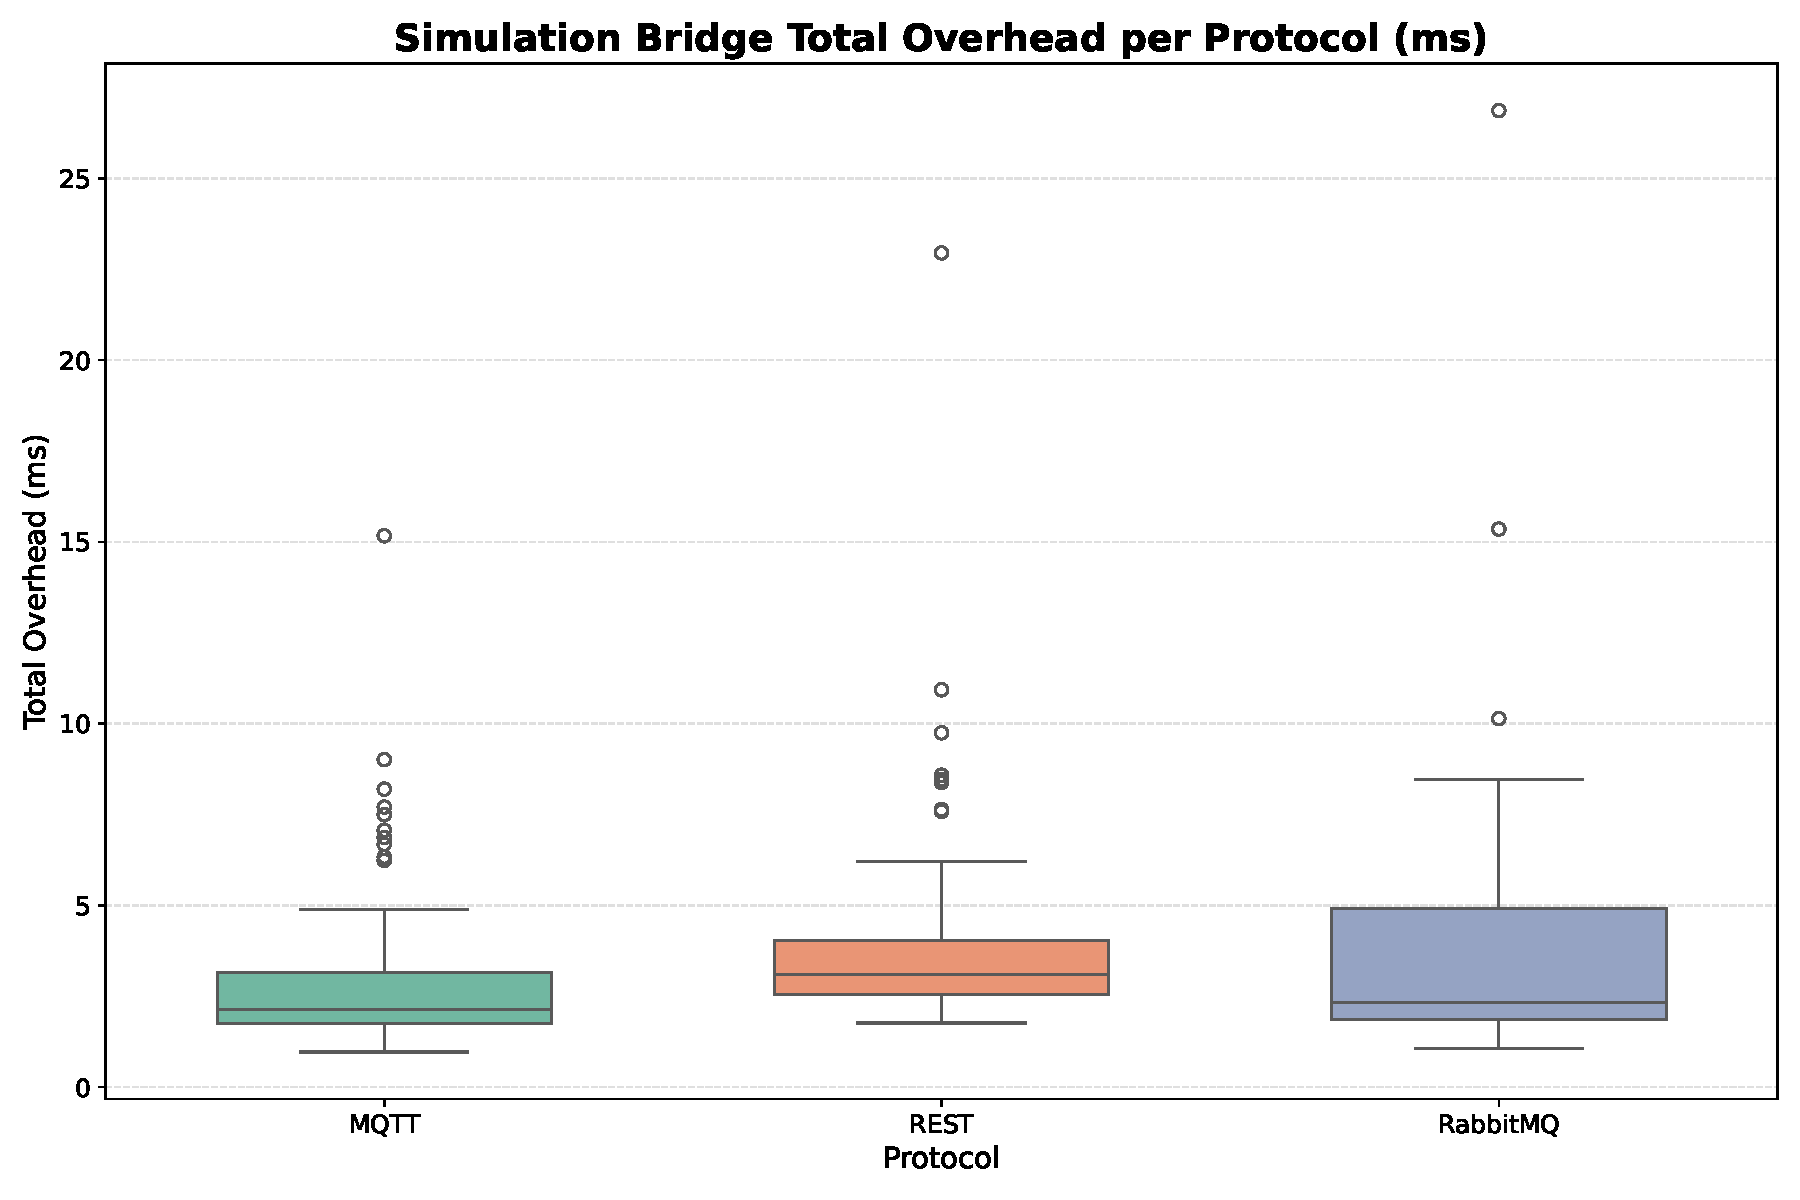
\includegraphics[width=0.9\columnwidth, trim=0in 0in 0in 0.4in, clip]{img/simulation_bridge_overhead_boxplot.pdf}
    \caption{The processing overhead in the core of the simulation bridge.}
    \label{fig:sim-bridge-overhead}
    %\vspace{-0.5cm}
\end{figure}    
\end{comment}

%%%%%%%%%%%%%%%%%%%%%%%%%%%%%%%%%%%%%%%%%%%%%%
\begin{figure*}[h]
    \centering
    \subfloat[The UR10e robotic arm in MatLab.]{
        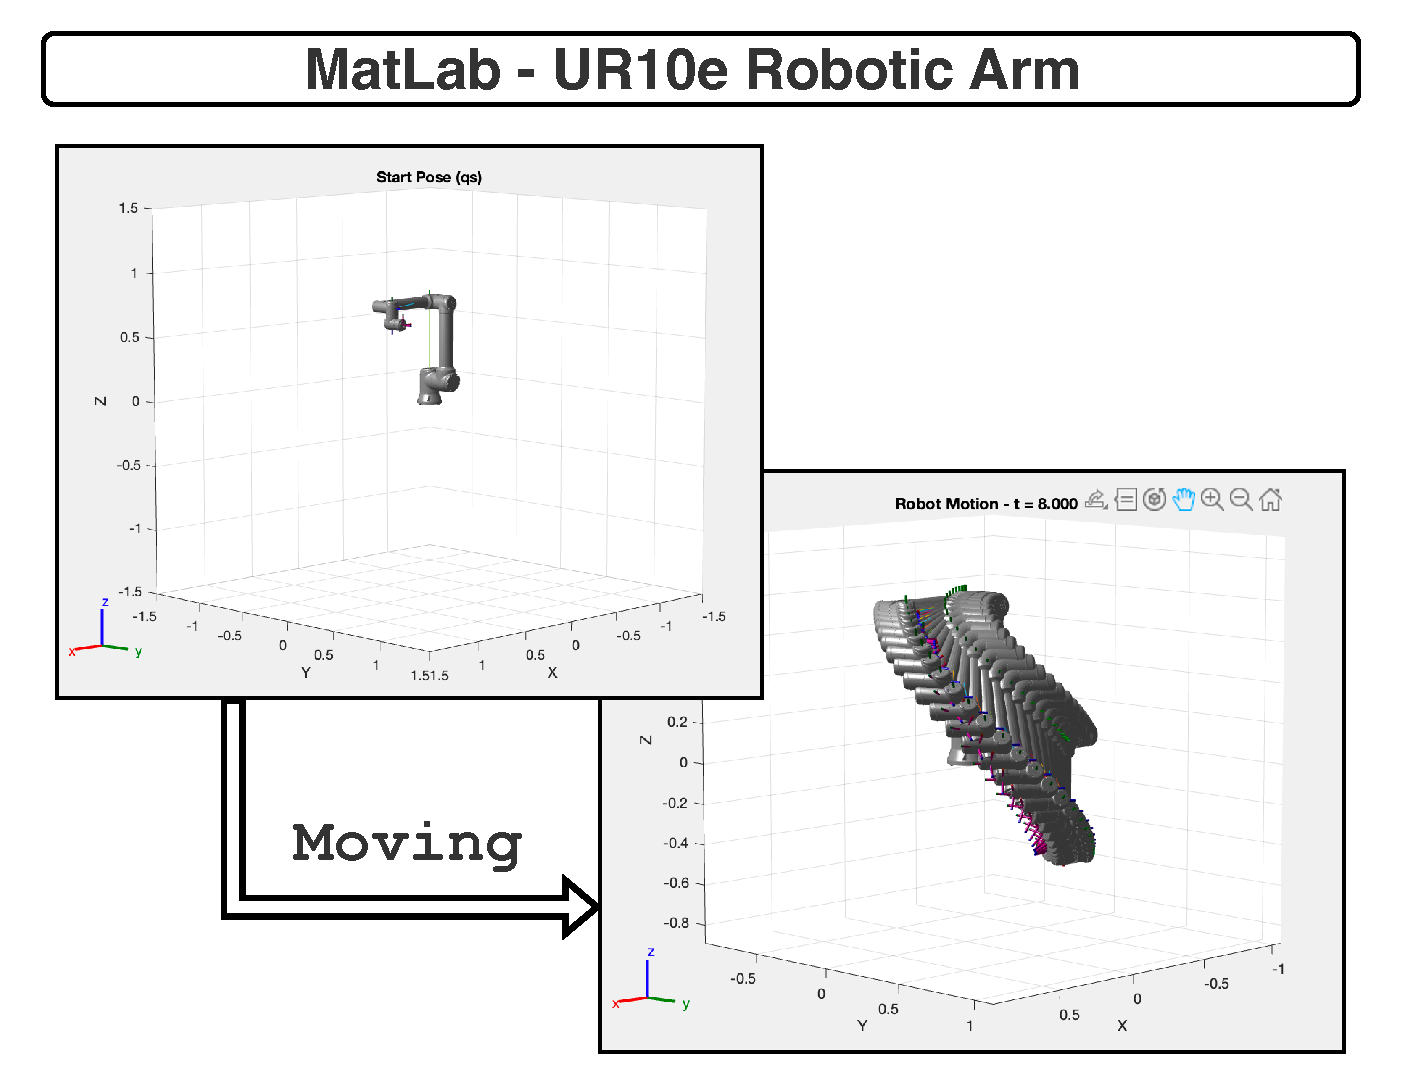
\includegraphics[width=0.465\linewidth]{img/matlab_pt.pdf}
        \label{fig:matlab_pt}
    }
    \hfill
    \subfloat[AnyLogic Microfactory simulation.]{
        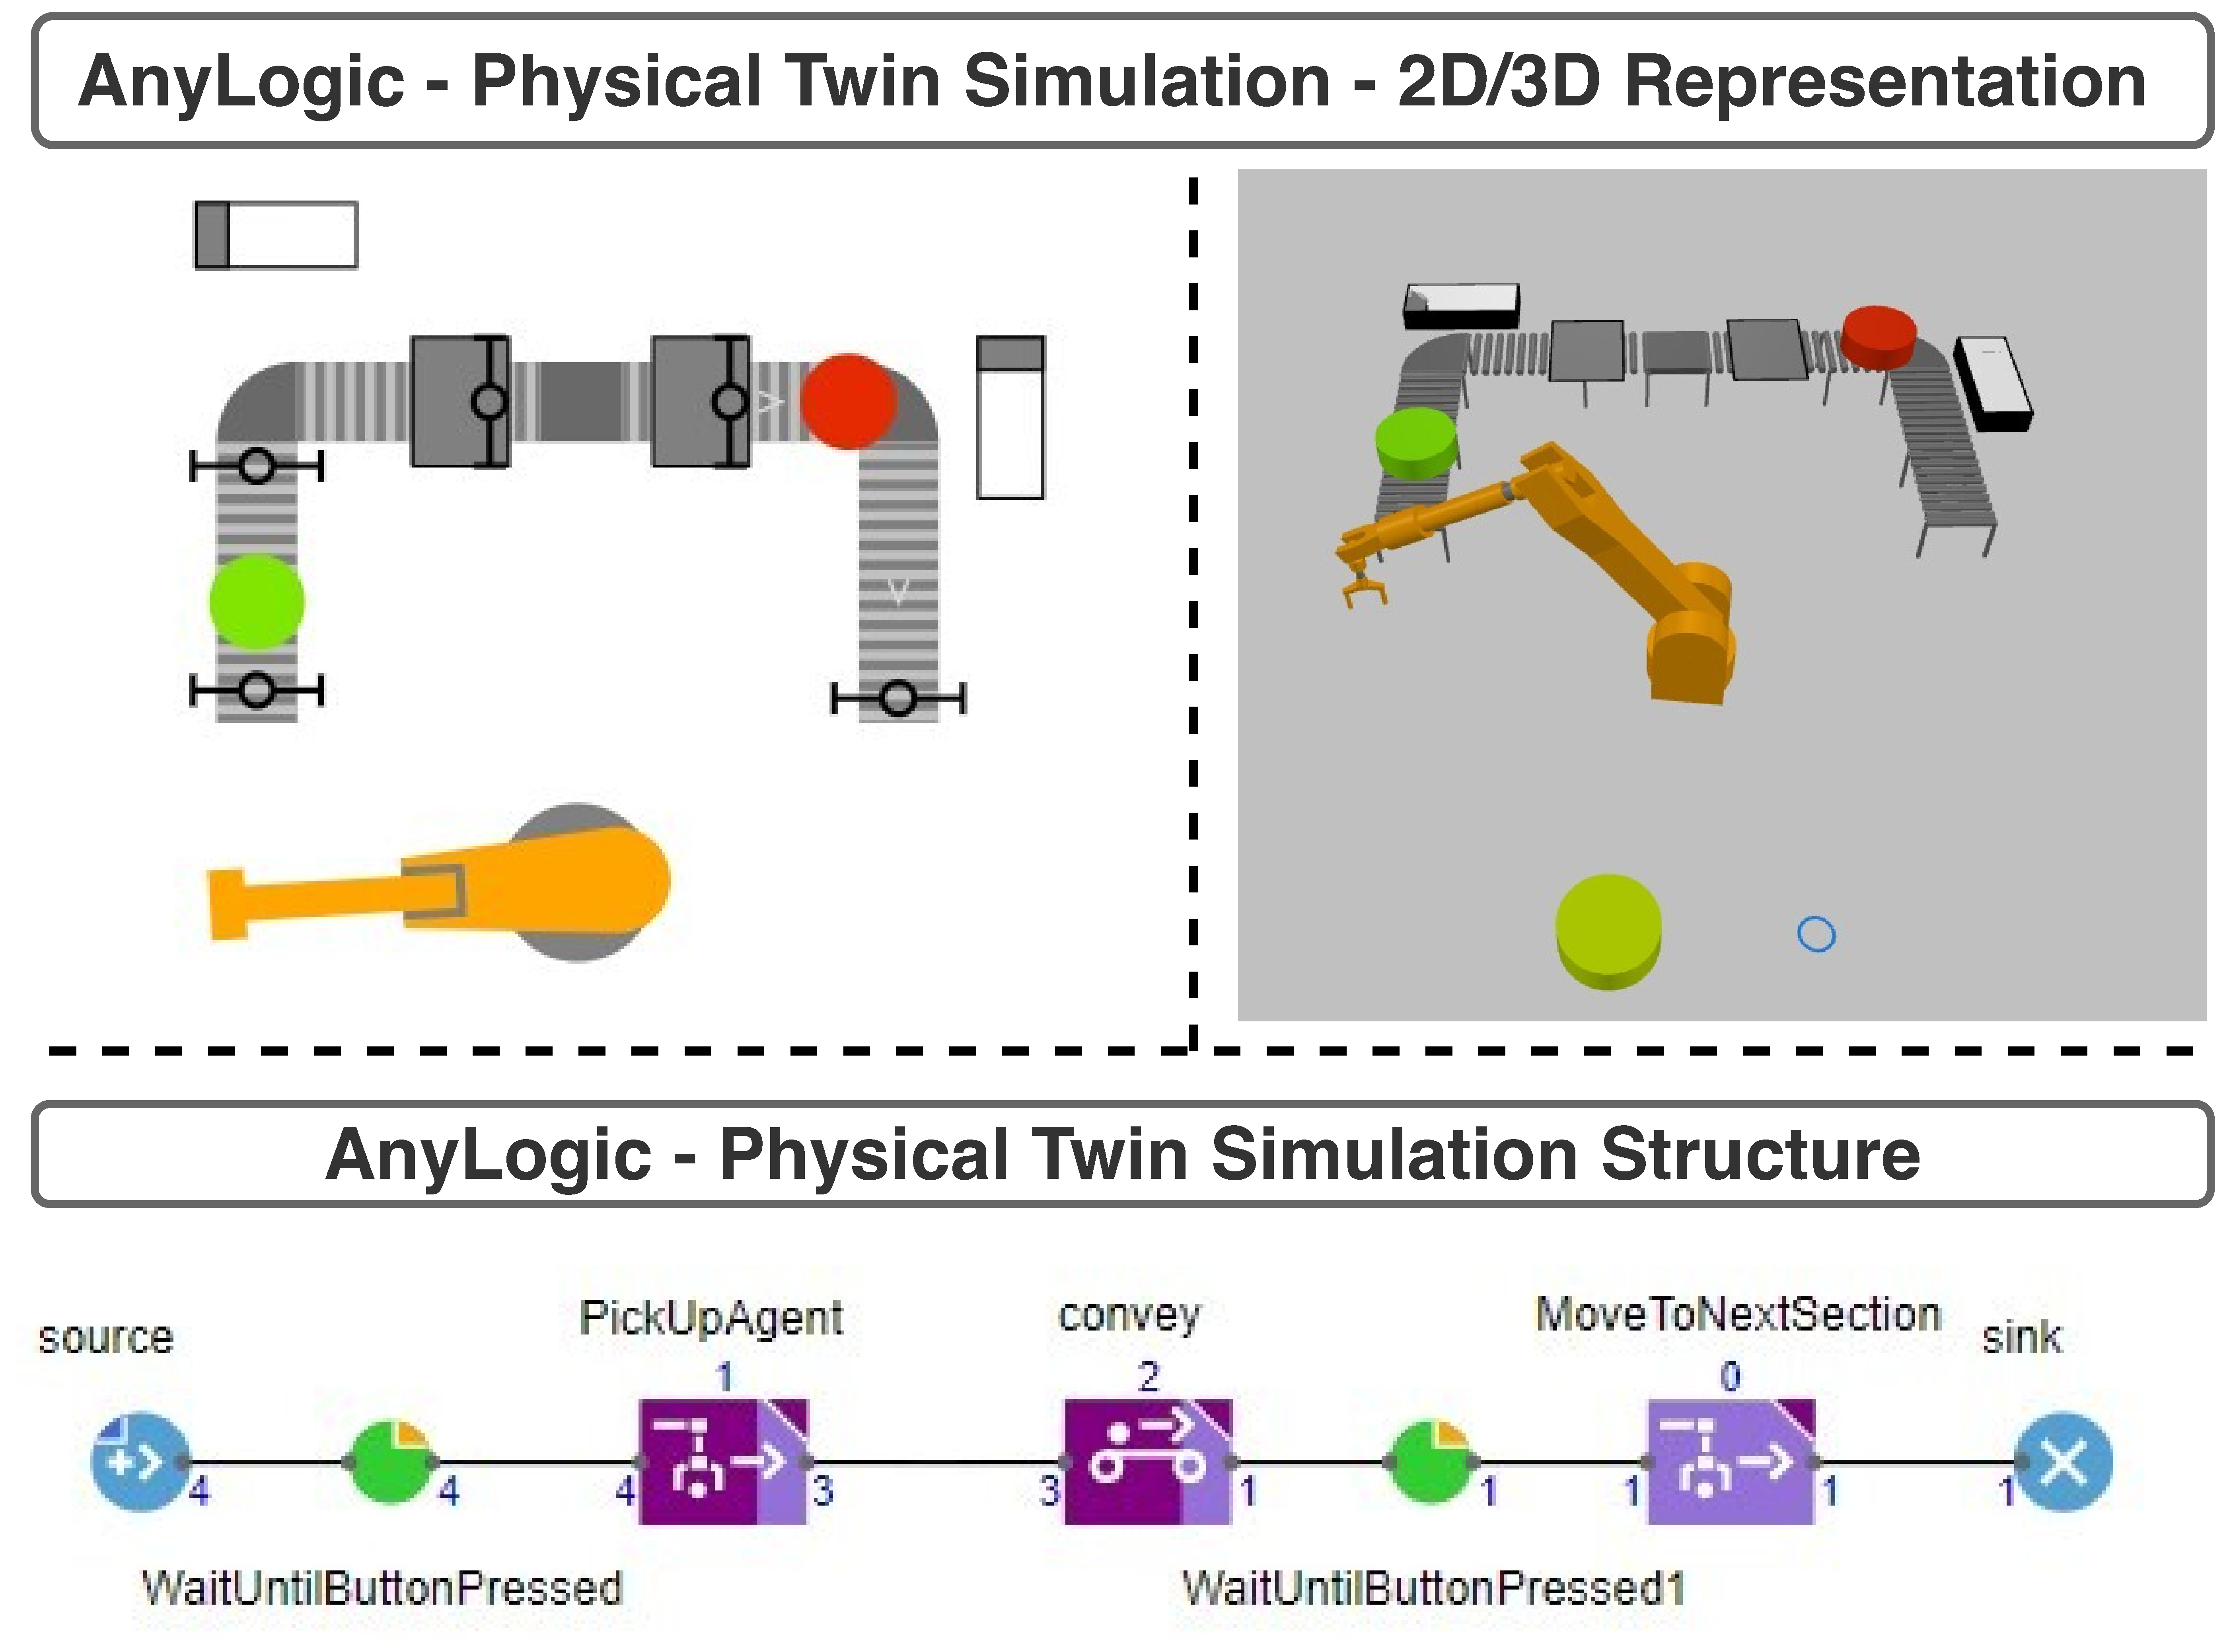
\includegraphics[width=0.48\linewidth]{img/any_logic_simple.pdf}
        \label{fig:any_logic_simple}
    }
    \caption{Simulated Physical Twins integrated with the Simulation Bridge.}
    \label{fig:physical_twin_simulations}
    \vspace{-0.5cm}
\end{figure*}
%%%%%%%%%%%%%%%%%%%%%%%%%%%%%%%%%%%%%%%%%%%%%%

\begin{table}[htbp]
\centering
\caption{Performance of DT-SB for different protocols.}
\label{tab:dt-sb_performance}
\renewcommand{\arraystretch}{1.5}
\begin{tabular}{p{0.3in}p{0.4in}p{0.3in}p{0.75in}p{0.75in}}
\hline
\textbf{Protocol} & \textbf{Overhead} & \textbf{STD} & \textbf{5\% Threshold} & \textbf{95\% Threshold} \\
\hline
MQTT & 2.47ms & 10.49ms & 1.69ms & 11.98ms \\
AMQP & 1.95ms & 0.99ms & 1.12ms & 3.69ms \\
REST & 4.63ms & 4.72ms & 2.92ms & 11.42ms \\
\hline
\end{tabular}
\vspace{-0.5cm}
\end{table}

% \begin{table}[htbp]
% \centering
% \caption{Performance comparison of DT simulation bridge for different protocol adapters. \textcolor{blue}{(The difference in values for REST/HTTP2.0 need to be explained.)}}
% \label{tab:dt-sb_performance}
% \renewcommand{\arraystretch}{1.5}
% \begin{tabular}{p{0.5in}p{0.5in}p{0.5in}p{0.5in}p{0.5in}}
% \hline
% \textbf{Protocol} & \textbf{Median Total Overhead (ms)} & \textbf{Standard Deviation (ms)} & \textbf{5\% Threshold (ms)} & \textbf{95\% Threshold (ms)} \\
% \hline
% MQTT & 2.47 & 10.49 & 1.69 & 11.98 \\
% AMQP & 1.95 & 0.99 & 1.12 & 3.69 \\
% REST (HTTP/2.0) & 4.63 & 4.72 & 2.92 & 11.42 \\
% \hline
% \end{tabular}
% \end{table}


\section{Experimental Evaluation}
\label{sec:experimental_evaluation}

To evaluate the performance of the proposed DT-SB and its integration with simulation agents, we conducted a series of experiments focusing on protocol overhead and agent-level performance on commercial computing hardware (MacBook Air Apple Silicon M2 processor and 8~GB of unified memory) with Python implementation of the proposed DT-SB \footnote{Simulation Bridge GitHub Repo: \url{https://github.com/INTO-CPS-Association/simulation-bridge}}. 

% All tests were executed on an Apple MacBook Air (2023) equipped with an Apple Silicon M2 processor and 8~GB of unified memory. MATLAB was natively installed on macOS, and Python profiling modules were used to gather performance metrics.

\subsection{Simulation Bridge Overhead}

\textbf{DT-SB Overhead}. The DT-SB was implemented to support multiple communication protocols on its north-bound interface (facing DTs), including MQTT, AMQP, and HTTP/2.0. Its south-bound interface (facing simulation agents) currently supports AMQP. We evaluated the processing time overhead introduced by the DT-SB core, explicitly excluding the contribution of individual protocol adapters.
Table \ref{tab:dt-sb_performance} shows the descriptive statistics of measured processing time overhead for MQTT, AMQP, and HTTP/2.0 protocol adapters.
These results confirm that DT-SB can reliably handle heterogeneous PAs with minimal latency in request forwarding and agent selection.
%These results indicate negligible performance differences across protocols and confirm that DT-SB can reliably handle heterogeneous DT communication channels with minimal latency in request forwarding and agent selection.

\textbf{Matlab Agent Overhead}.
% A dedicated MATLAB agent was developed to interface the DT-SB with MATLAB simulations. 
To assess the performance of the MATLAB agent independently of simulation model complexity, we used lightweight test cases to isolate the agent's intrinsic processing overhead. Each simulation request was assigned a unique \textit{Request ID}, enabling precise tracking of request-response cycles. For streaming mode experiments, different time steps were used to vary the frequency of data exchange, simulating increased communication loads.
The overhead refers to the time spent by the agent to process a simulation request, excluding MATLAB startup time and simulation runtime. This metric captures the cost of request parsing, file operations, and inter-process communication. In batch mode, the agent exhibited a mean overhead of 2.7~ms. In streaming mode, the mean overhead was 3.7~ms. Table~\ref{tab:matlab-streaming} reports the measured overhead for different streaming frequencies, showing that agent performance remains stable across varying time steps. These findings confirm that $SA_{\text{MATLAB}}$ introduces minimal latency, making it suitable for both batch and real-time streaming applications.

\begin{table}[h!]
\centering
\caption{Matlab Agent's overhead for different frequencies.}
\label{tab:matlab-streaming}
\begin{tabular}{lcccccc}
\hline
\textbf{Streaming Frequency (ms)} & 10 & 50 & 70 & 100 & 150 & 200 \\ 
\hline
\textbf{Agent Overhead (ms)} & 2.2 & 4.1 & 5.6 & 4.9 & 3.2 & 3.0 \\ 
\hline
\end{tabular}
\end{table}

\textbf{Anylogic Agent Overhead}. To evaluate the performance of the AnyLogic agent a dedicated testing campaign was conducted to measure the system’s intrinsic overhead, independently of simulation model complexity aligned with the MATLAB agent analysis. The simulation used for the experiment is shown in Figure~\ref{fig:any_logic_simple}. The AnyLogic model employed is event-based, meaning that the simulation flow is internally controlled and does not rely on a fixed time step, unlike Table~\ref{tab:matlab-streaming}, which reports the MATLAB agent’s overhead at different frequencies. To ensure comparability with previous analyses, the simulation was executed at various run-time speeds (1x, 2x, 5x, 10x, 25x, 50x). The results show an extremely low and stable average overhead, ranging from 3.4~ms to 8.6~ms across different streaming configurations, as reported in Table~\ref{tab:anylogic-streaming}. These findings confirm that $SA_{\text{AnyLogic}}$ introduces negligible latency, making it suitable for real-time streaming applications.

\begin{table}[h!]
\centering
\caption{AnyLogic Agent's overhead at different execution speeds.}
\label{tab:anylogic-streaming}
\begin{tabular}{lcccccc}
\hline
\textbf{Execution Speed} & 1x & 2x & 5x & 10x & 25x & 50x \\ 
\hline
\textbf{Agent Overhead (ms)} & 8.6 & 4.9 & 8.3 & 3.4 & 5.3 & 3.6 \\ 
\hline
\end{tabular}
\end{table}



\begin{comment}
\begin{table}[h!]
\centering
\caption{Matlab Agent's overhead for different frequencies.}
\label{tab:matlab-streaming}
\begin{tabular}{lcccccc}
\hline
\textbf{Streaming Frequency (ms)} & 10 & 50 & 70 & 100 & 150 & 200 \\ 
\hline
\textbf{Agent Overhead (ms)} & 2.2 & 4.1 & 5.6 & 4.9 & 3.2 & 3.0 \\ 
\hline
\end{tabular}
\end{table}
\end{comment}

\begin{comment}
\paragraph{Startup to Total Duration Ratio}
This metric expresses the portion of total request time spent initializing MATLAB. A high ratio indicates significant startup overhead.
\begin{center}
\begin{tabular}{|l|c|}
\hline
\textbf{Request ID} & \textbf{Startup / Total Duration Ratio} \\
\hline
streaming\_10ms  & 0.6143 \\
streaming\_50ms  & 0.5652 \\
streaming\_70ms  & 0.3907 \\
streaming\_100ms & 0.4352 \\
streaming\_150ms & 0.5369 \\
streaming\_200ms & 0.5906 \\
batch            & 0.1747 \\
\hline
\end{tabular}
\end{center}
\textbf{Mean Ratio:} \texttt{0.4725}    

\paragraph{System Resource Utilization}
The average resource usage during execution was as follows:
\begin{itemize}
    \item \textbf{Mean CPU Usage:} \texttt{94.30\%}
    \item \textbf{Mean Memory RSS:} \texttt{25.31 MB}
\end{itemize}
\end{comment}

% \begin{figure}[ht]
%     \centering
%     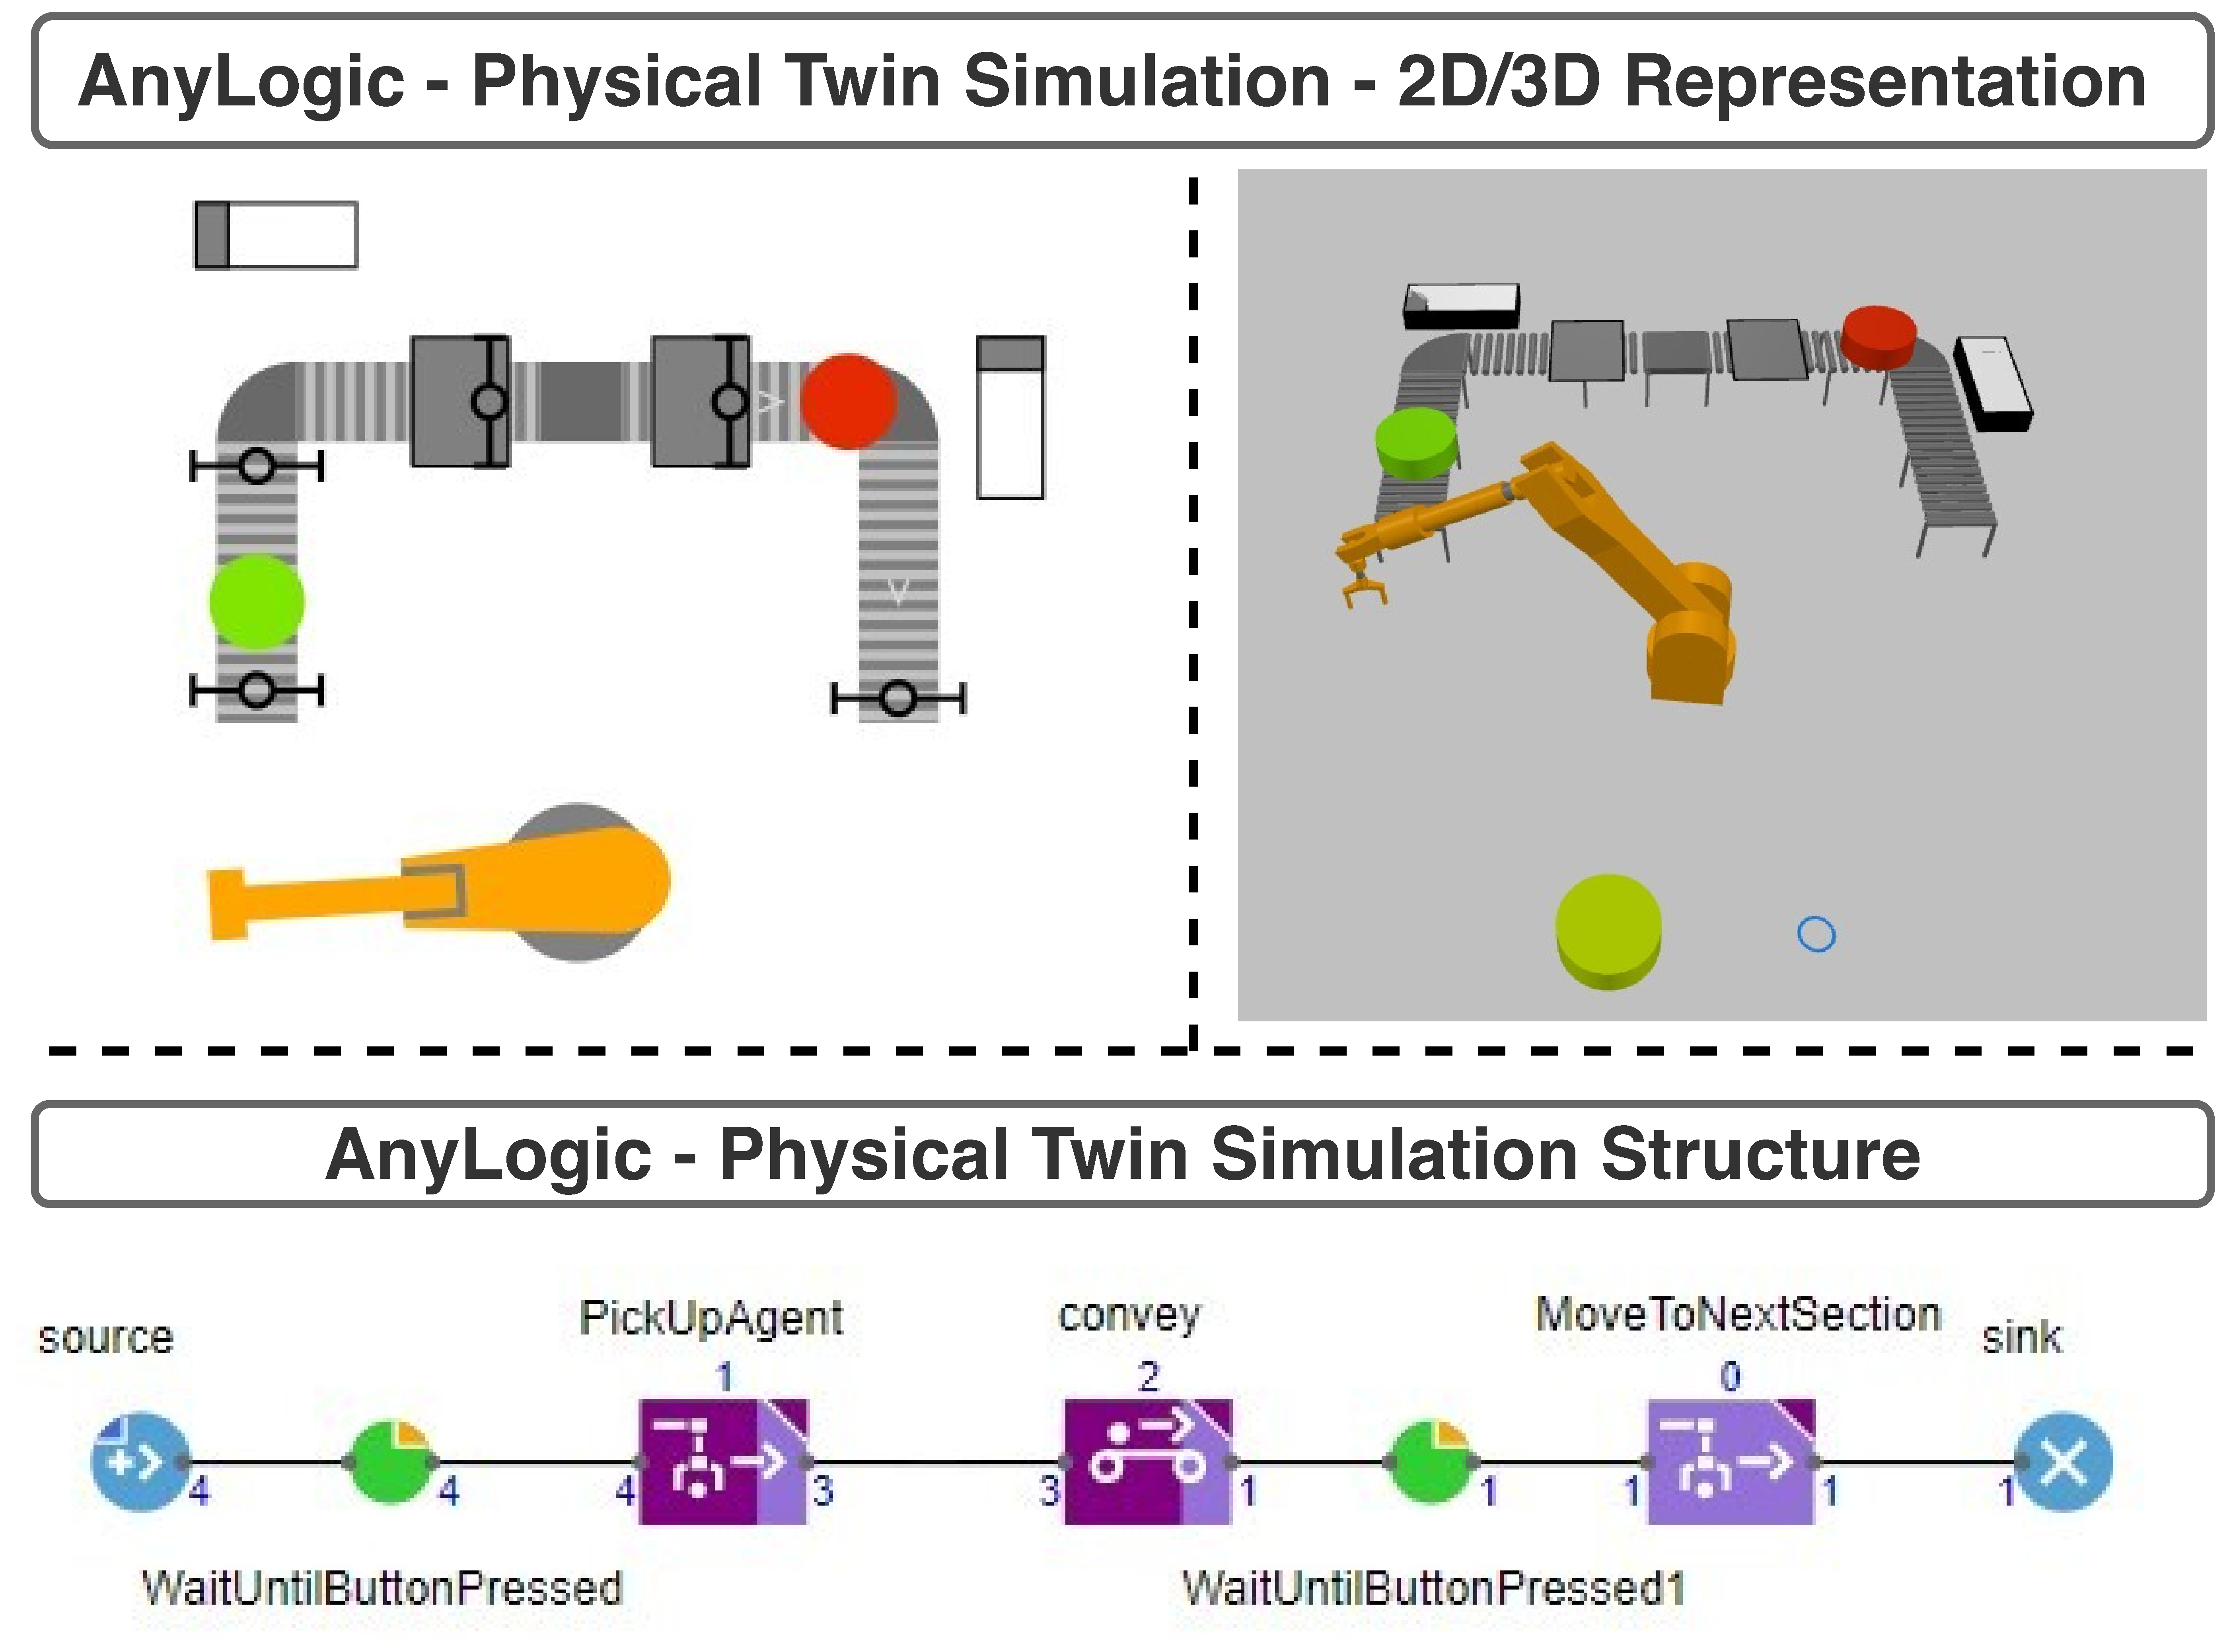
\includegraphics[width=0.9\columnwidth]{img/any_logic_simple.pdf}
%     \caption{AnyLogic PT simulation.}
%     %\Description{AnyLogic PT simulation.}
%     \label{fig:any_logic_simple}
%     \vspace{-0.5cm}
% \end{figure}

\subsection{Physical Twin Simulations}

To validate and analyze the proposed Simulation Bridge framework and the integration with DTs, two simulation environments were developed to emulate distinct aspects of the PTs behaviors: one in \textit{MATLAB/Simulink}, focusing on robotic motion control and kinematics, and one in \textit{AnyLogic}, modeling a microfactory scenario for system-level DT integration and communication assessment.

The first simulation involves a Universal Robots UR10e robotic arm executing a smooth point-to-point motion in joint space as depicted in Figure \ref{fig:matlab_pt}. The objective is to move the robot from an initial joint configuration to a target configuration within a specified time, following an optimally smooth trajectory and employing a simple closed-loop controller to track this trajectory. To ensure smooth motion, a fifth-order (quintic) polynomial trajectory was defined for each of the robot’s six joints. A quintic polynomial has six coefficients, allowing the imposition of six boundary conditions (initial and final position, velocity, and acceleration). This ensures continuity of the first and second derivatives—velocity and acceleration—throughout the entire motion.

The robotic simulation was implemented using the Robotics System Toolbox and a rigid-body model of the UR10e with gravity enabled. At each time step, the control law computed a new joint velocity command, and joint angles were updated via simple Euler integration. This iterative process continued until the planned trajectory duration elapsed. Completion was detected when the final joint configuration error dropped below a predefined negligible threshold, ensuring accurate convergence to the target configuration.

The second simulated environment was developed using the DT-SB integrated agent within \textit{AnyLogic} to support DT creation for a Microfactory scenario. The model represents an indexed production line comprising a conveyor, multiple workstations, and a robotic arm responsible for handling parts between loading and unloading areas, as illustrated in Figure~\ref{fig:any_logic_simple}. 

% The environment was built using the \textit{AnyLogic Material Handling Library}\footnote{AnyLogic Material Handling Library: \url{https://www.anylogic.com/features/libraries/material-handling-library/}}.

The two-dimensional model includes conveyors capable of reporting operational status, photocells detecting product passage, and transfer stations with custom switches emulating pusher mechanisms. Workstations are equipped with virtual actuators that communicate their operational state, while the central robot, modeled via the \textit{Robot} element, manages item positioning and state updates. Process logic is implemented using a block-diagram approach: agents are generated by a \textit{Source} block, controlled by a \textit{Hold} block linked to user interface commands, processed by a \textit{ProcessByRobot} block, transferred using a \textit{Convey} block, and finally removed by a \textit{Sink} block. 

Together, these simulation environments provided a controlled and complementary validation setup for the proposed approach. The MATLAB/Simulink model enabled low-level evaluation of motion control and trajectory tracking, while the AnyLogic microfactory scenario assessed system-level communication, synchronization, and interoperability. This combination demonstrated the framework’s flexibility in connecting diverse simulation domains within a unified DT integration architecture.

% This setup enables the DT to process data as if originating from real PTs. Communication performance was assessed by measuring the latency of bidirectional data exchange via MQTT. The average measured communication overhead from AnyLogic to the DT was \(6.5~\mathrm{ms}\) with a standard deviation of \(10~\mathrm{ms}\). Overall, the AnyLogic simulation provides a controlled and repeatable environment for DT testing, supporting experimentation on PT conditions, communication protocols, synchronization strategies, and cyber-physical system (CPS) integration.



% This use-case involves a Universal Robots UR10e robotic arm executing a smooth point-to-point motion in joint space. The objective is to move the robot from an initial joint configuration to a target configuration within a specified time, following an optimally smooth trajectory and using a simple closed-loop controller to track this trajectory.

% To ensure smooth motion, we employed a 5th-order (quintic) polynomial trajectory for each of the robot’s six joints. A quintic polynomial has six coefficients, which allows imposing six boundary conditions (start and end position, velocity, and acceleration) – exactly what is needed to guarantee continuous first and second derivatives (velocity and acceleration) throughout the motion. 

% The simulation was implemented in MATLAB/Simulink (Robotics System Toolbox) using a UR10e rigid-body model with gravity enabled. A fixed integration time-step of \(\Delta t = 5 ms\) was used to update the robot’s joint states. At each time step, the control law above was applied to compute a new joint velocity command, and the joint angles were updated as (simple Euler integration). This process was repeated until the planned trajectory time elapsed and the robot had effectively reached the goal. To determine completion, we set a very small threshold on the final error: the loop stops only once ensuring the final joint configuration is achieved with negligible error.

% The simulated environment was developed using the DT-SB integrated agent for AnyLogic to support DT creation for a microfactory scenario, featuring an indexed line with a conveyor, workstations, and a robot handling parts between loading areas, as shown in Figure~\ref{fig:any_logic_simple}.

% built with the AnyLogic Material Handling Library\footnote{AnyLogic Material Handling Library: \url{https://www.anylogic.com/features/libraries/material-handling-library/}}, 

% The two-dimensional model, includes conveyors reporting status, photocells detecting product passage, and transfer stations with custom switches emulating pushers. Workstations have virtual actuators reporting status, and the central robot, modeled via the \textit{Robot} element, manages item positioning and state updates. The simulation integrates all key entities and focuses on assessing the communication overhead of bidirectional data exchange with the DT via the DT-SB.

% Process logic uses a block diagram: agents are generated by a \textit{Source} block, controlled by a \textit{Hold} block linked to UI buttons, processed by a \textit{ProcessByRobot} block, moved via a \textit{Convey} block, and removed by a \textit{Sink} block. The DT processes data as if from real PTs. The measured communication overhead from AnyLogic to the DT via MQTT averaged $6.5\,\mathrm{ms}$ with a standard deviation of $10\,\mathrm{ms}$.

% This setup offers a controlled, repeatable environment for testing DTs, supporting experimentation with PT conditions, communication protocols, synchronization, and CPS integration strategies.


% The simulated environment was developed using the DT-SB integrated agent for AnyLogic to enable and support the creation of DTs for a microfactory scenario. This scenario features an indexed line with a conveyor, multiple workstations, and a robot that moves pieces between loading areas, as illustrated in Figure~\ref{fig:any_logic_simple}, showing both the simulation structure and the 2D/3D visualizations.

% The two-dimensional model of the indexed line was developed using elements from the AnyLogic Material Handling Library\footnote{AnyLogic Material Handling Library: \url{https://www.anylogic.com/features/libraries/material-handling-library/}}. 
% The conveyors simulate the physical transport system and report their operational status, while photocells detect and signal the passage of products at predefined positions. In the absence of dedicated pushers, transfer stations combined with a custom-designed switch emulate their functionality, sending position change messages to the Simulation Bridge. 
% The workstations are equipped with virtual actuators that report machine status and process progress. The robot at the center of the microfactory is modeled using the AnyLogic \textit{Robot} element, which handles item positioning and transmits state updates, such as item pick-up events. 
% The target simulation integrated all core production entities---the conveyor, robotic arm, workstations, photocells, and product flow---and focused on evaluating the communication overhead of bidirectional data exchange between the DT and the simulation environment through the DT Simulation Bridge.

% The process logic is implemented as a block diagram. Simulation agents are generated by a \textit{Source} block, controlled by a \textit{Hold} block linked to UI buttons that govern robot operation. Items are processed by a \textit{ProcessByRobot} block defining pick-and-place tasks, moved along conveyor paths via a \textit{Convey} block, and finally removed by a \textit{Sink} block. 
% In this setup, the DT processes data as if it were sent from real Physical Twins, although these are simulated. The measured communication overhead, from the AnyLogic simulation environment to the DT via MQTT, resulted in an average delay of approximately $6.5 \,\mathrm{ms}$, with a standard deviation of about $10 \,\mathrm{ms}$.

% This integrated industrial simulation, combined with the DT-SB, provides a controlled, repeatable environment for developing and testing DTs. It supports experimentation with different PT conditions, communication protocols, synchronization mechanisms, and integration strategies for physical and CPSs.

